\section*{1D 系統架構}

\subsection*{設計理念}

我們以鋼球平衡台作為專題的主體,然後寫程式驅動雷射測距感測器當鋼球遠離時platfor,當鋼球靠近時platform放下,重複此動作直至鋼球平衡台平衡。

\begin{figure}[h!]
    \centering
    \begin{minipage}[b]{0.45\textwidth}
        \centering
        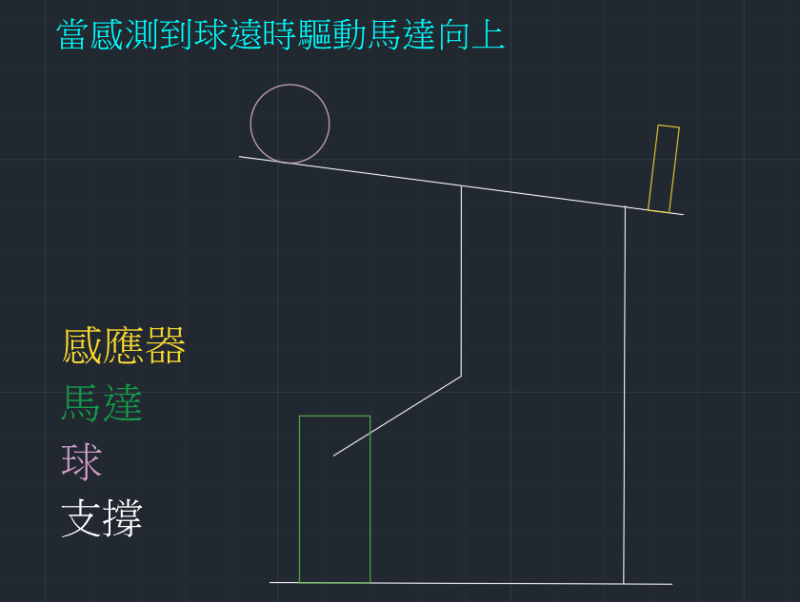
\includegraphics[width=\textwidth,height=0.22\textheight]{./../images/螢幕擷取畫面 2024-05-22 181158.png}
        \caption{2D草圖(1)}
    \end{minipage}
    \hfill
    \begin{minipage}[b]{0.45\textwidth}
        \centering
        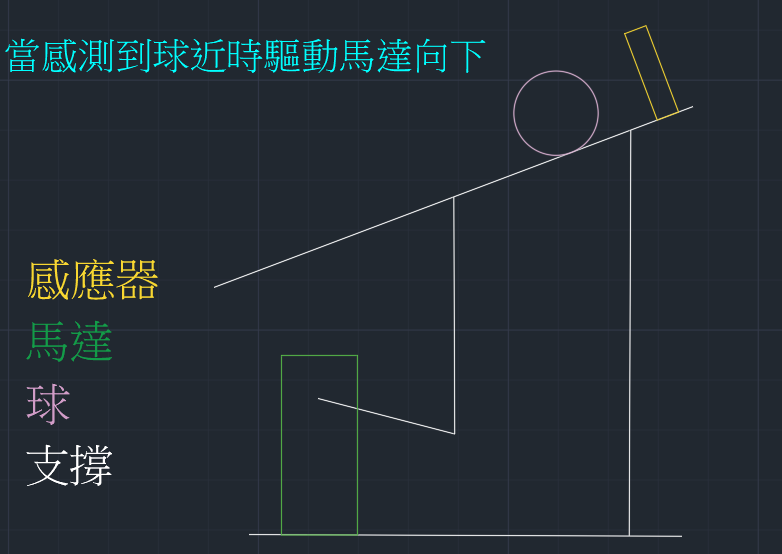
\includegraphics[width=\textwidth,height=0.22\textheight]{./../images/螢幕擷取畫面 2024-05-22 180925.png} 
        \caption{2D草圖(2)}
    \end{minipage}
\end{figure}

\subsection*{馬達角度所對應之平台角度關係}

\begin{figure}[htbp]
    \centering
    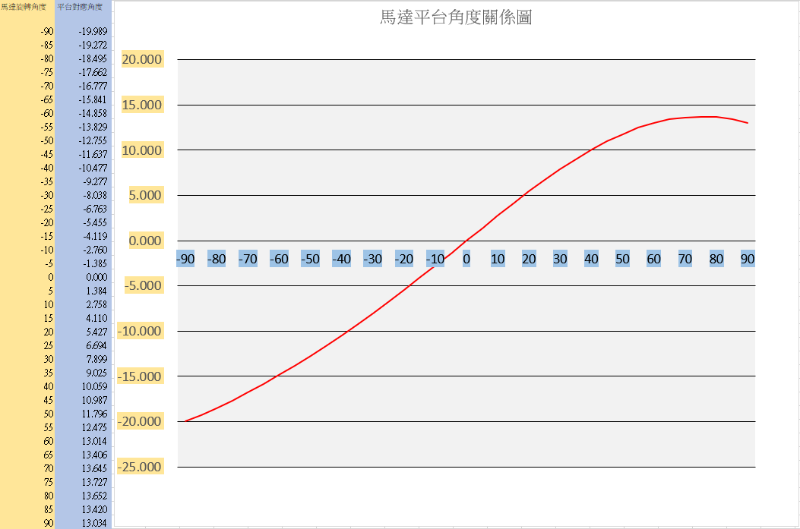
\includegraphics[width=1\textwidth]{./../images/6-1-50}
    \caption{馬達角度關係圖}
\end{figure}

使用 SolidWorks 2023 進行繪圖。
\begin{figure}[htbp]
    \centering
    
\includegraphics[width=0.5\textwidth]{./../images/6-1-1}
    \caption{SOLIDWORKS}
\end{figure}

\subsection*{platform}

第一版本鋼球平衡台的 platform 軌道長度為 200mm 整體的寬度為 30mm 並給定深度填料 11mm。

\begin{figure}[h!]
    \centering
    \begin{minipage}[b]{0.6\textwidth}
        \centering
        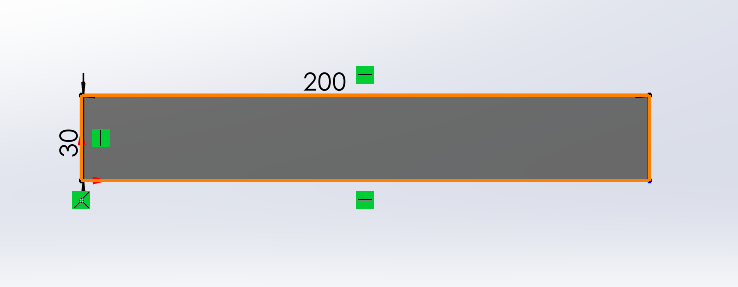
\includegraphics[width=\textwidth,height=0.22\textheight]{./../images/6-1-11}
        \caption{PLATFORM草圖 (1)}
        \label{fig:platform}
    \end{minipage}
    \hfill
    \begin{minipage}[b]{0.3\textwidth}
        \centering
        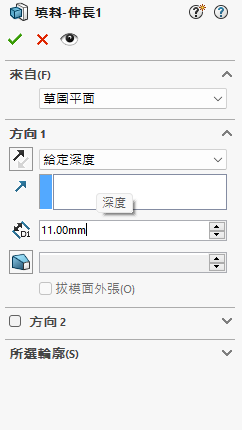
\includegraphics[width=\textwidth,height=0.3\textheight]{./../images/6-1-12} 
        \caption{編輯特徵(1)}
        \label{fig:feature1}
    \end{minipage}
\end{figure}
軌道上方寬度為 8.5mm,下方為 7.2mm,深 4mm並將紅圈處深伸長除料選擇完全貫穿。

下方配合處長 30mm 寬 6mm,繪製好圖形草圖。

給予尺寸後伸長填料 25mm。

填料完成後再圖形上畫一個 2.9mm 的小孔並進行伸長除料以便與其他零件配合。

第一版 platform 完成圖。

\textbf{修改部分}

軌道上方增加長 26.2mm 寬 2mm 的貫穿凹槽,用於放置感應器。

下方接合處新增 R10 圓角。

最終 Platform 零件圖。

\textbf{3D 列印成果}

\subsection*{base}

第一版 Base 底的長為 237mm 寬為 150mm。

在底板長 55mm 寬 54mm 處繪製一個 12mm $\times$ 12mm 的方形柱並向上填料 100mm。

在方柱上方繪製一個長 30.28mm 寬 20 的長方體然後在長方體上畫直徑 20mm 的半圓最後在圓的中心繪製一個 3.98mm 的小孔最後在長方體上畫一個長 30mm 寬 10.8mm 的小長方體伸長除料選擇完全貫穿方便與上方 platform 配合。

在距離方柱中心長 129mm 寬 25mm 處繪製一個長 31mm 寬 20mm 向上填料 7mm 的小平台用來定位馬達。

並且在兩邊加畫底 15mm 高 45mm 的三角形支撐架防止馬達晃動。

第一版 base 完成圖。

\textbf{修改部分}

底部去除浪費的部分改以長 165.6mm 圓直徑 22.35mm 的直狹槽代替。

為了好收納將左方柱子拔除留下一凹槽方便後續配合及螺絲孔。

最終 base 完成圖。

\textbf{3D 列印成果}

\subsection*{support}

從底座拔除的部分目的好收納尺寸都沒有改變。

最終 support 完成圖。

\textbf{3D 列印成果}

\subsection*{link}

上方連結處與 support 尺寸一致皆為長 30.28mm 寬 20 的長方體然後在長方體上畫直徑 20mm 的半圓最後在圓的中心繪製一個 3.98mm 的小孔最後在長方體上畫一個長 30mm 寬 10.8mm 的小長方體伸長除料選擇完全貫穿方便與上方 platform 配合。

下方為 12mm $\times$ 12mm 的方柱並填料 68mm 方便與馬達進行配合。

最終 link 完成圖。

\textbf{3D 列印成果}

\subsection*{assemble}

組合完成圖。

\subsection*{驅動方式}

使用金屬齒輪伺服馬達配合程式控制平台,程式放置於 6-3。


